
\section*{Downtime Actions}
\DefineNamedColor{named}{eclipsered}{rgb}{0.486,0.566,0.582}
\definecolor{tablecolor}{named}{eclipsered}

%General overview of downtime:

\begin{itemize}
    \itembox Base unit of downtime is usually \SI{1}{week}.
    \itembox Each week, player may perform exactly \num{1} of the given downtime actions.
\end{itemize}

\bigskip

\begin{eptable}{ l | X }
   \epheader{2}{Downtime Actions}
   Acquire / Make Things & See Table.\\
   Change Motivation &  Pretty easy.\\
   Fulfill Responsibilities &  Wrap up, may initiate Contact.\\
   Manage Rep &  See Table.\\
   Mod Yourself &  See Table.\\
   Train \& Improve &  See Table.\\
   Gain Positive Ego Trait &  Should be story based, costs RP.\\
   Improve Aptitudes &  See rule book.\\
   Improve Skills &  \num{5} per week, or \num{1} per week when skill >= \num{60}.\\
   Increase Flex &  May not exceed 3.\\
   Learn Language & Usually takes months; only if exposed.\\
   Learn PSI Sleight & One \SI{1}{RP} per sleight.\\
   Lose Negative Ego Trait & Takes months preparation, some impossible.\\
   Specialize & Minimum skill level \num{30}.\\
\end{eptable}


\begin{figure}[h!]%
   \centering
   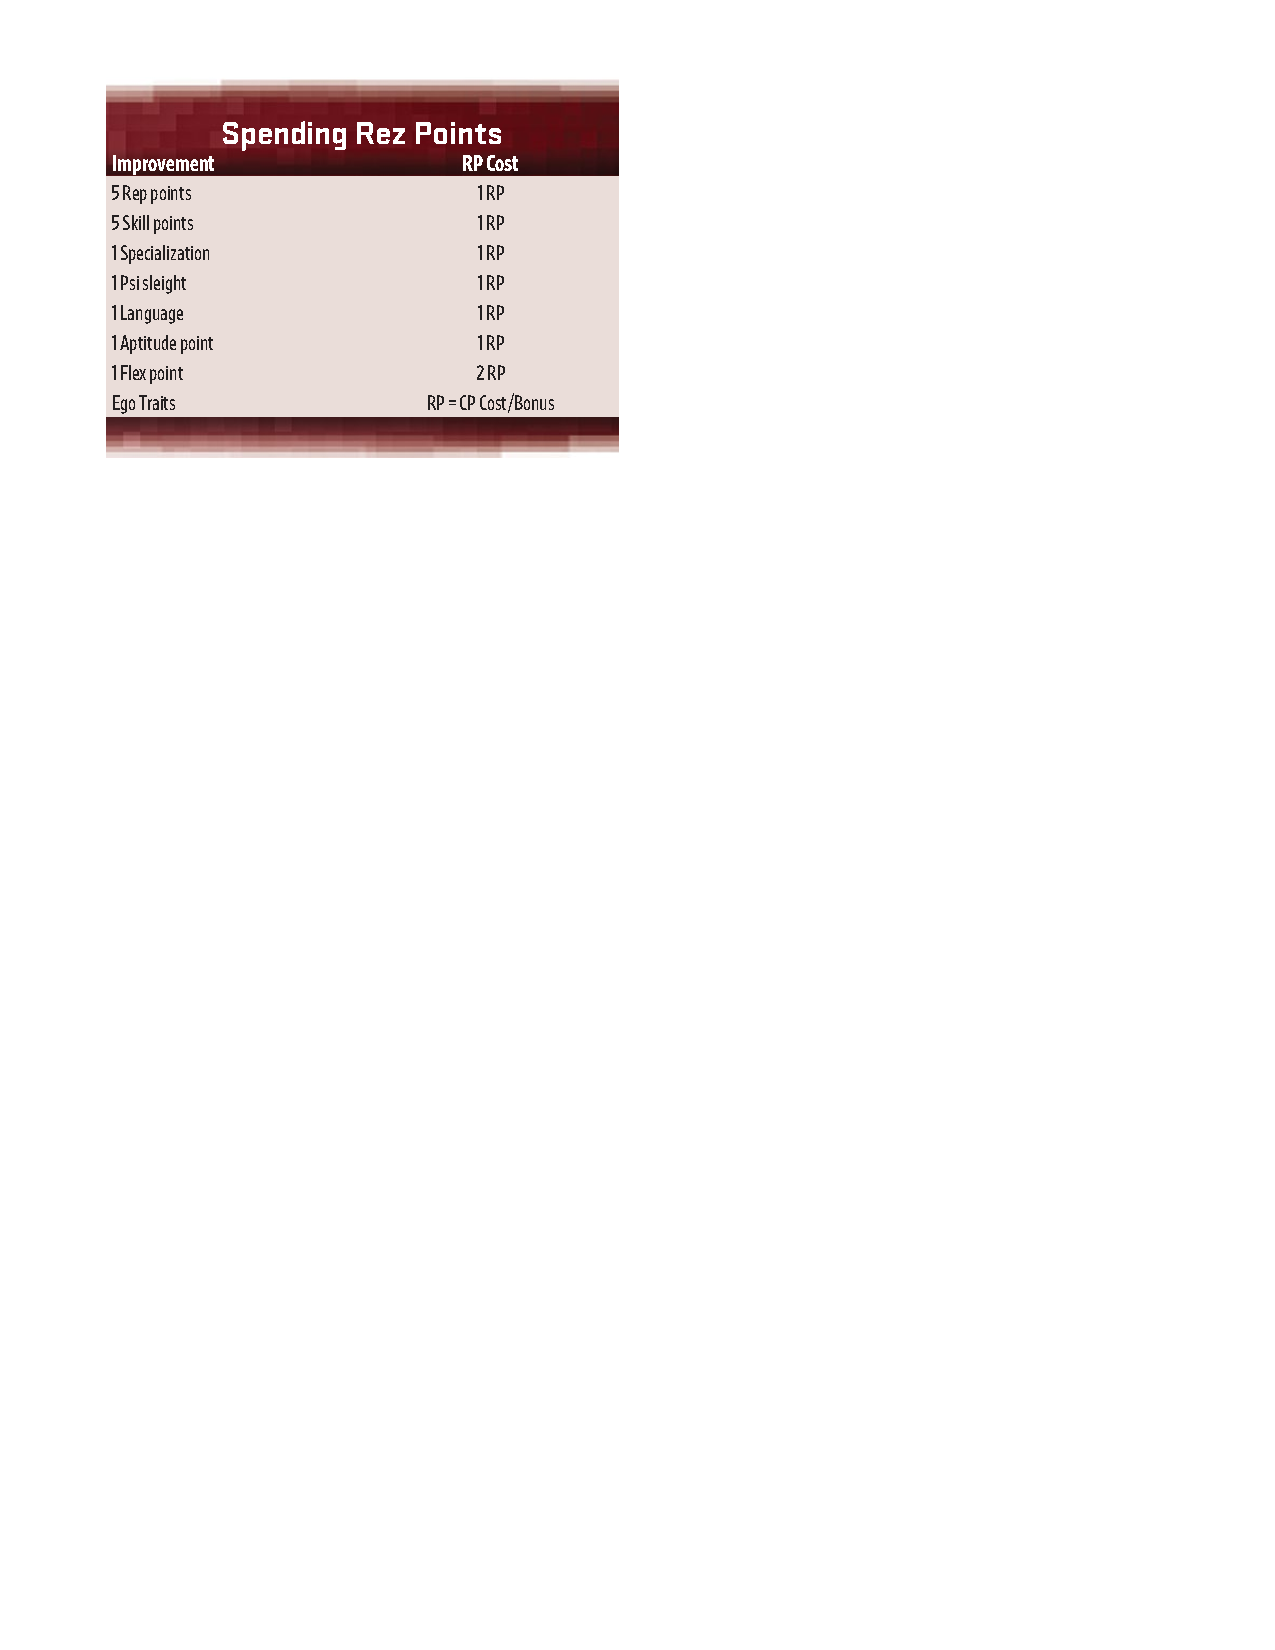
\includegraphics[scale=0.9]{gfx/downtime-rez}%
\end{figure}%
